\documentclass[tikz]{standalone}
\usepackage{pgfplots}
\begin{document}

\usetikzlibrary{decorations.pathreplacing}
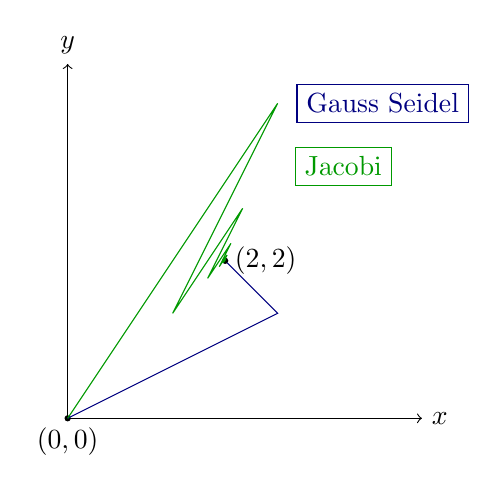
\begin{tikzpicture}[shift={(10.0,0.0)}]

  \definecolor{gscol}{rgb}{0.0,0.0,0.5}
  \definecolor{jcol}{rgb}{0.0,0.6,0.0}


  \draw[->] (0.0, 0.0) -- (4.5,0.0) node[right] {$x$};
  \draw[->] (0.0, 0.0) -- (0.0,4.5) node[above] {$y$};

  \fill (0.0,0.0) circle[radius=0.04] node[below] {$(0,0)$};
  \fill (2.0,2.0) circle[radius=0.04] node[right] {$(2,2)$};


% next step
%  2.666667, 1.333333,
% next step
%  2.222222, 1.777778,
% next step
%  2.074074, 1.925926,
% next step
%  2.024692, 1.975308,

  % jacobi
  \draw[gscol]
  (0.0,0.0) --
  (2.666667, 1.333333) --
  (2.222222, 1.777778) --
  (2.074074, 1.925926) --
  (2.024692, 1.975308) --
  (2.024692, 1.975308);

  \draw[jcol]
  (0.0,0.0) --
  (2.666667, 4.000000) --
  (1.333333, 1.333333) --
  (2.222222, 2.666667) --
  (1.777778, 1.777778) --
  (2.074074, 2.222222) --
  (1.925926, 1.925926) --
  (2.024692, 2.074074) --
  (1.975309, 1.975308) --
  (2.008231, 2.024691) --
  (1.991770, 1.991769) --
  (1.991770, 1.991769);

  \node[draw,gscol] at (4.0,4.0) {Gauss Seidel};

  \node[draw,jcol] at (3.5,3.2) {Jacobi};

\end{tikzpicture}

\end{document}
